\section{问题分析与总体思路}

\subsection{并行收益为何受到数据流限制}
依赖图中的独立分支提供并行执行机会，但计算量均衡并不等于完成时间均衡。一个核心即使承担较少计算，也可能长时间等待前驱数据；多个核心同时搬入时，又会竞争同一 DDR 带宽池。将一条大张量依赖切开，既增加搬运工作量，也可能把原本连续的计算链变成跨核等待链。判断一个切分是否值得，需要把计算、依赖与通信放在同一时间尺度上比较。

弱连通分量给出了较自然的起点：不同分量之间不存在计算依赖，保持分量完整可以避免切断其内部生产--消费关系。然而，分量可能共同读取同一个外部输入，分量内部也可能超过核内缓存容量。因此，完整分量装箱减少的是由内部切分引入的边界代价，并不意味着总 DDR 流量为零。若最大分量占据大部分工作量，还必须考察其内部并行结构。

输入图的另一项差异来自计算管道。相同的操作周期总和可能对应不同的矩阵、向量工作量组成；若仅按总周期分核，两个核心可能分别拥堵在不同管道，或一个核心的单管道成为瓶颈。本文在分量和子图层面保留双管道负载，再通过通信与依赖估计比较可行划分。

\subsection{从任务边界到数据驻留和读取时序}
场景 A 中，切图边界直接决定 Task 边界，减少不必要边界有助于降低重复搬运。场景 B 中，同核子图可以连续复用数据，优化重点转向哪些操作应被安排在同一核心。把共享张量的消费者集中起来能够减少跨核读取，却也可能延迟张量的最后一次使用，使缓存长期被占用。本文以张量的首次出现和末次使用估计驻留区间，将容量压力引入候选排序。

只读 Cache 又增加了一项时间条件：第二次读取必须在首次读取完成之后、条目被淘汰之前发射，才能形成命中。共享输入很多并不足以说明收益大；如果各核同时发起首次读取，或共享张量很快被新条目挤出，潜在复用不会转化为带宽收益。第三问因而继承场景 B 的分核与驻留分析，并进一步展开读写请求的事件时序。

\begin{figure}[htbp]
\centering
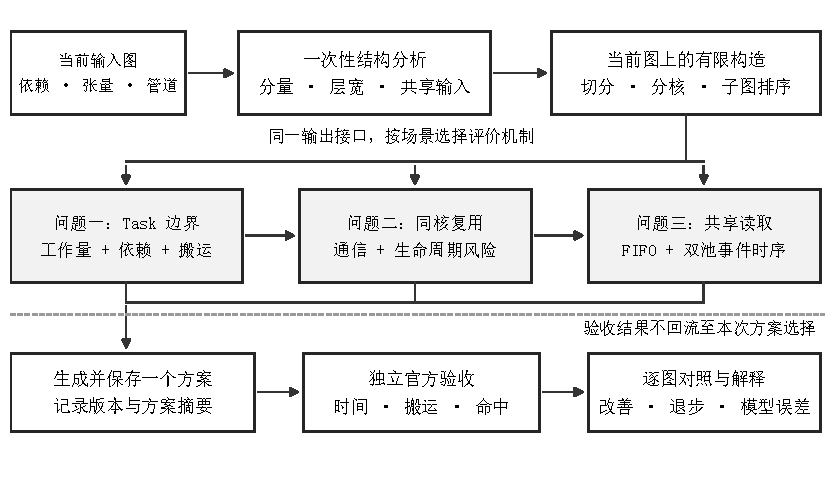
\includegraphics[width=\linewidth]{figures/fig2_1.pdf}
\caption{三问共用的决策过程及逐层增加的运行机制。输入结构在每个图上重新计算；实线连接求解所用信息，底部表示方案保存后的独立验收。图中节点为建模环节，不代表实际执行时间。}
\label{fig:overall}
\end{figure}

\subsection{已有方法的启发与本题的实现范围}
深度学习编译器研究强调图表示、调度和目标硬件之间的配合\cite{Liu2025}。经典最长作业优先分配与列表调度分别提供了负载分散和关键路径优先的构造思路\cite{Graham1969,Topcuoglu2002}。这些方法能够低成本产生初始方案，但本题的任务时间会随切图、缓存换出和共享带宽竞争变化，不能直接套用独立定长作业模型的性能界。

基于性能建模的调度研究说明，估计模型的用途在于把任务和资源信息转化为可比较的决策依据\cite{Yang2025}。本文采用有限种结构构造，并让统一模型对当前图产生的方案进行排序。候选是一次求解过程中的中间决策，最终接口仍接收一个图并输出一个方案。构造数量受到显式限制，避免把大部分时间用于反复调用耗时的完整模拟。

MAGIS 将图优化与调度中的延迟、内存开销联合考虑\cite{Chen2024}，Timeloop 用架构和数据流模型分析加速器的存储与执行代价\cite{Parashar2019}。本文从中吸收张量生命周期分析和资源服务量建模的思路，具体实现保持题目原计算图与固定硬件配置。既不进行算子融合、计算复制或重计算，也不引入题目未给出的张量分块与映射维度。

三个问题具有完工时间与额外搬运量两个评价方向。本文将完工时间置于主要位置，用搬运量和驻留风险修正时间代理或打破并列。当前算法采用确定性构造与评分选择，未执行非支配排序或种群进化；后文公式和伪代码均围绕这一实际求解过程展开。
